% arara: indent: {overwrite: yes}
\section{Лабораторная 2}

\subsection{Условие}

\textbf{Согласно варианту 10:}
\begin{enumerate}
	\item Пуассона – $\Pi(\lambda), \lambda = 0.7$; Геометрическое – $G(p), p = 0.2$;
	\item Бернулли – $Bi(1, p), p = 0.75$; Пуассона – $\Pi(\lambda), \lambda = 1$;
\end{enumerate}

Смоделировать дискретную случайную величину. Исследовать точность моделирования.

\begin{enumerate}
	\item Осуществить моделирование $n = 1000$ реализаций СВ из заданных дискретных распределений;
	\item Вывести на экран несмещённые оценки математического ожидания и дисперсии, сравнить их с истинными значениями;
	\item Для каждой из случайных величин построить свой $\chi^{2}$-критйрий Пирсона с уровнем значимости $\varepsilon = 0.05$. Проверить, что вероятность ошибки I рода стремится к 0.05;
	\item Осуществить проверку каждой из сгенерированных выборок каждым из построенных критериев.
\end{enumerate}

\subsection{Теория}
\subsubsection{Датчик случайной величины распределения Пуассона}

\textbf{Распределение Пуассона} -  распределение дискретного типа случайной величины, представляющей собой число событий, произошедших за фиксированное время, при условии, что данные события происходят с некоторой фиксированной средней интенсивностью и независимо друг от друга.\\

\textbf{Функция распределения:}
\begin{equation}
	\frac{\Gamma (k+1,\lambda)}{k!}.
\end{equation}

\textbf{Функция вероятности:}
\begin{equation}
	\frac{e^{-\lambda}\lambda^{k}}{k!}.
\end{equation}

\textbf{Математическое ожидание:} $\lambda$.\\

\textbf{Дисперсия:} $\lambda$.

\paragraph{Алгоритм моделирования:}\
\\

При моделировании будем использовать свойство пуассоновского процесса, состоящего в том, что
время ожидания появления события имеет показательное распределение:

\begin{equation}
	F_{\tau}(t) = 1 - e^{-\lambda t}.
\end{equation}

Следовательно, последовательность наступления событий в пуассоновском процессе можно задать через \textit{последовательность времён ожидания} этих событий. При этом надо проверять, чтобы суммарное время \textit{суммарное время ожидания событий в цепочке не превышала единицы}.

Последовательность времён ожидания можно получить методом обратных функций:

\begin{equation}
	\tau_{i} = - \frac{1}{\lambda} \cdot \ln(1-u_{i}),
	\label{pre_poisson_generator:ref}
\end{equation}

где $u_{i} = rnd(1)$ - \textit{случайные числа}, т.е. значения случайной величины (СВ), равномерно распределённой на [0, 1].

Последовательность (\ref{pre_poisson_generator:ref}) следует продолжать, пока не нарушается условие:

\begin{equation}
	\sum_{i=1}^{j}\tau_{i} = \sum_{i=1}^{j}(-\frac{1}{\lambda} \cdot \ln(1-u_{i} \leqslant 1.
	\label{pre_poisson_condition:ref}
\end{equation}

Максимально возможное количество слагаемых в сумме (\ref{pre_poisson_condition:ref}) и будет равно числу появления событий в данной серии, т.е. эти числа и есть значения случайной величины, имеющей распределение Пуассона.

\begin{enumerate}
	\item Во-первых, в (\ref{pre_poisson_condition:ref}) заменим выражение $1-u_{i}$ просто на $u_{i}$, поскольку они имеют один и тот же закон распределения;
	\item Во-вторых, избавимся от операций логарифмирования в каждом слагаемом, для чего пропотенциируем выражение (\ref{pre_poisson_condition:ref}).
\end{enumerate}

Таким образом, определим случайную величину:
\begin{equation}
	\xi = max \left\lbrace j : \prod_{i}^{j} u_{i} \geqslant e^{-\lambda} \right\rbrace, \lambda > 0,
\end{equation}

которая описывается распределением Пуассона. Элемент выборки можно получить последовательно увеличивая число членов $(j)$ в произведении до тех пор, пока не нарушится условие:

\begin{equation}
	\prod_{i}^{j} u_{i} \geqslant e^{-\lambda},
\end{equation}

максимальное значение $(j)$, удовлетворяющее этому условию и есть очередное значение случайной величины.\\


\textbf{\textit{Программа создания выборки:}}
\begin{figure}[h!]
	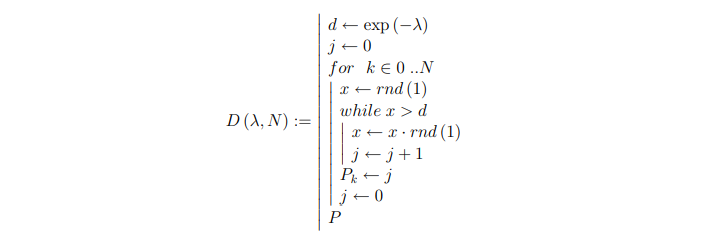
\includegraphics [width=\textwidth] {pseudo_algorithm_poisson_generator.png}
	\caption{Псевдоалгоритм генерации СВ распределения Пуассона.}
	\label{fig:pirson_critical_values}
\end{figure}

\subsubsection{Датчик случайной величины геометрического распределения}

Под \textbf{Геометрическим распределением} в теории вероятностей подразумевают одно из двух распределений дискретной случайной величины:\

\begin{itemize}
	\item распределение вероятностей случайной величины $X$ равное номеру первого ``успеха'' в серии испытания Бернулли и принимающей значения $n = 1,2,3,\ldots$;
	\item распределение вероятностей случайной величины $Y = X - 1$, равное количеству ``неудач'' до первого ``успеха'' и принимающей значения $n = 0,1,2,\ldots$.
\end{itemize}

\textbf{Функция распределения:}
\begin{equation}
	1 - q^{n+1}.
\end{equation}

\textbf{Функция вероятности:}
\begin{equation}
	q^{n}p.
\end{equation}

\textbf{Математическое ожидание:}
\begin{equation}
	\frac{q}{p}.
\end{equation}

\textbf{Дисперсия:}
\begin{equation}
	\frac{q}{p^{2}}.
\end{equation}

\paragraph{Алгоритм моделирования:}\
\

\begin{enumerate}
	\item Моделирование реализации $\alpha$ БСВ;
	\item Принятие решения о том, что реализация $\xi$ является значением $x$, определяемым соотношением:
	      \begin{equation}
		      x = \left[ \frac{\ln \alpha}{\ln q} \right],
	      \end{equation}
	      где $[z]$ - округление числа $z$ в большую сторону до ближайшего целого значения.
\end{enumerate}

\subsubsection{Датчик случайной величины распределения Бернулли}

\textbf{Распределение Бернулли} - дискретное распределение вероятностей, моделирующее случайный эксперимент произвольной природы, при заранее известной вероятности успеха или неудачи.:\

\textbf{Функция распределения:}
\begin{equation}
	\begin{cases}{}
		0, k < 0             \\
		q, 0 \leqslant k < 1 \\
		1, k \geqslant 1     \\
	\end{cases}.
\end{equation}

\textbf{Функция вероятности:}
\begin{equation}
	\begin{cases}{}
		q, k = 0 \\
		p, k = 1 \\
	\end{cases}.
\end{equation}

\textbf{Математическое ожидание:}
\begin{equation}
	p.
\end{equation}

\textbf{Дисперсия:}
\begin{equation}
	pq.
\end{equation}

\paragraph{Алгоритм моделирования:}\
\

\begin{enumerate}
	\item Моделирование реализации $\alpha$ БСВ;
	\item Принятие решения о том, что реализация $\xi$ является значением $x$, определяемым по правилу:
	      \begin{equation}
		      x =
		      \begin{cases}{}
			      1, \alpha \leqslant p \\
			      0, \alpha > p         \\
		      \end{cases}.
	      \end{equation}
\end{enumerate}

\subsection{Код программы}

\lstinputlisting[language=Python]{./lab_2/lab2.py}

\subsection{Результат выполнения}

\begin{figure}[H]
	\centering
	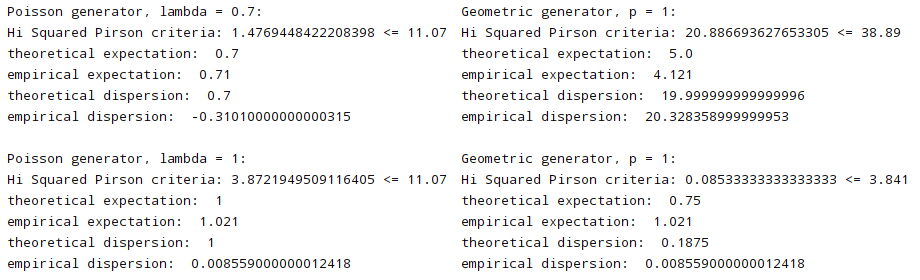
\includegraphics [width=\textwidth] {results_lab_2.jpg}
	\label{fig:results}
	\caption{Результат выполнения программы: проверка критерием согласия Пирсона и подсчёт несмещённых оценок математического ожидания и дисперсии.}
\end{figure}

\begin{figure}[!h]
	\centering
	\begin{subfigure}[b]{0.45\textwidth}
		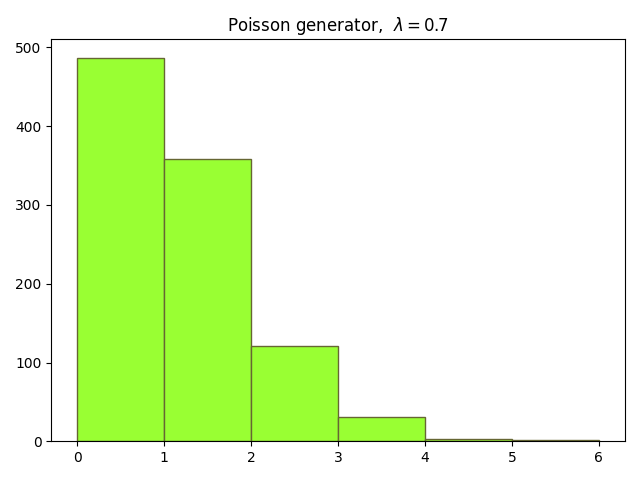
\includegraphics[width=\textwidth]{poisson_generator_l07.png}
		\caption{Диаграмма выборки, полученной генератором распределения Пуассона при $\lambda = 0.7$.}
	\end{subfigure}
	\hfill
	\begin{subfigure}[b]{0.45\textwidth}
		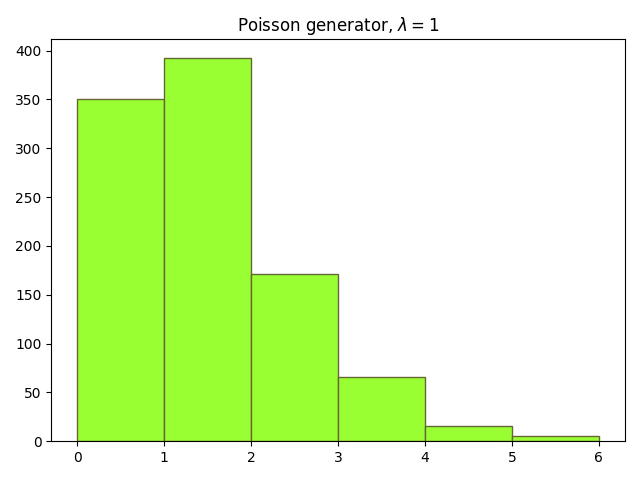
\includegraphics[width=\textwidth]{poisson_generator_l1.png}
		\caption{Диаграмма выборки, полученной генератором распределения Пуассона при $\lambda = 1$.}
	\end{subfigure}
	\\
	\begin{subfigure}[b]{0.45\textwidth}
		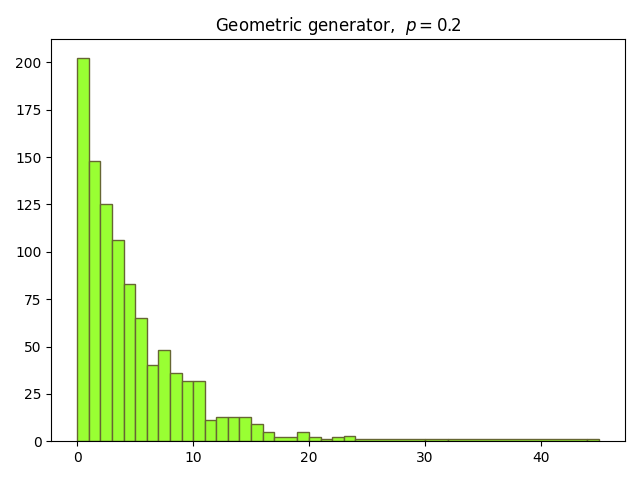
\includegraphics[width=\textwidth]{geometric_generator.png}
		\caption{Диаграмма выборки, полученной генератором геометрического распределения.}
	\end{subfigure}
	\hfill
	\begin{subfigure}[b]{0.45\textwidth}
		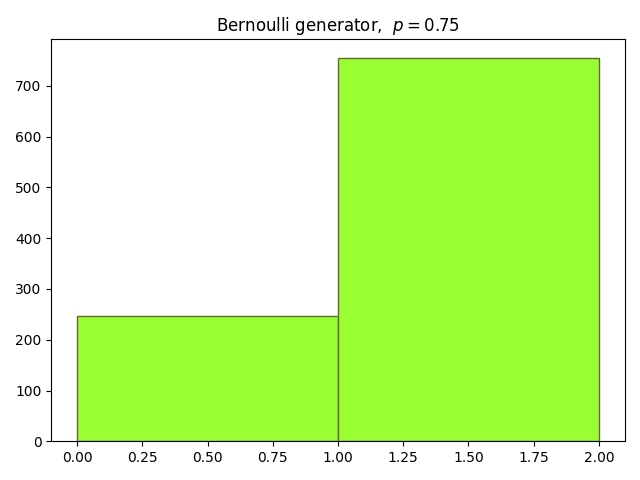
\includegraphics[width=\textwidth]{bernoulli_generator.png}
		\caption{Диаграмма выборки, полученной генератором распределения Бернулли.}
	\end{subfigure}
\end{figure}
